\chapter{Introduction}

The internet, as we know it today, heavily relies on the use of the HTTP protocol. Not only is it
used by web browsers to download and otherwise interact with websites, it also serves as a transport
medium for use with REST web APIs or technologies such as gRPC and GraphQL\@.

Currently, the latest published version of the protocol is HTTP/2 defined in RFC 7540 from 2015.
HTTP/2 improved on its predecessor HTTP/1.1 by introducing features such as request multiplexing
over a single TCP connection, header compression and the server-push feature, allowing it to
significantly reduce loading times of web pages and generally improve the efficiency of the web.

Currently, some limiting factors of HTTP/2 can be traced to the TCP protocol used on the
transport layer. Combination of request multiplexing and TCP's guaranteed delivery leads to a
problem where the loss of a TCP packet from one request will delay the transmission of other
requests. This is known as \textit{head-of-line blocking}.

Most of the web connections now use HTTPS instead of HTTP for security reasons. Establishment of
HTTPS connection requires first establishing the TCP connection via the three-way handshake.
Following that is the TLS handshake negotiating connection encryption. This process combined
requires several round trips before the first packet with an HTTP request can be sent.

Above mentioned and other problems are addressed in the HTTP/2's successor HTTP/3, which is
currently still in the draft stage. Because these problems are not caused by HTTP itself, but rather
the transport protocol underneath, HTTP/3 essentially replaces TCP and TLS layer with brand new
UDP-based named QUIC\@. Although QUIC is developed in parallel with HTTP/3, it is a general-purpose
transport protocol that can be used as a transport medium for other higher level protocols. The
relationship between protocols on HTTP/2 and HTTP/3 stacks are depicted in
figure~\ref{fig:http2-vs-http3-stack}.

\begin{figure}[h]\label{fig:http2-vs-http3-stack}
  \centering
  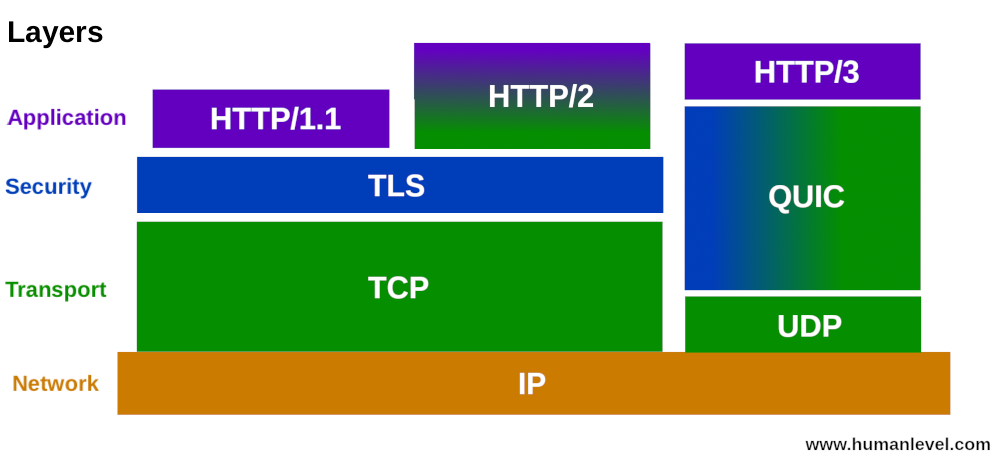
\includegraphics[width=\textwidth]{img/01-pile-http-protocol}
  \todo{Redraw this without HTTP/1.1 in inkscape}
  \caption{Comparison between HTTP/2 and HTTP/3 protocol stacks}
\end{figure}

The main improvements of QUIC over TCP+TLS can be summarized in following points:

\begin{itemize}
  \item \textit{Stream multiplexing} ---
    QUIC provides abstraction of multiple streams multiplexed on a single connection at the
    transport level. And because loss detection and retransmission is implemented at the QUIC layer,
    rather than UDP, the protocol does not exhibit the \textit{head-of-line blocking} problem
    discussed previously.

  \item \textit{Faster connection establishment} ---
    QUIC combines TCP-like three-way-handshake and TLS 1.3 handshake together, requiring fewer
    round-trips to establish connections and thus reducing latency. QUIC also supports TLS 1.3 Zero
    Round Trip Time Resumption (0-RTT)
    \todo{Explanation: https://blog.cloudflare.com/introducing-0-rtt/}, allowing it to send user data
    with the very first packet.

  \item \textit{Always encrypted} ---
    Because TLS handshake is part of connection establishment, the QUIC connection is always encrypted.

  \item \textit{Connection migration} ---
    QUIC identifies the connection by its ID rather than the peer's address. This allows clients on
    mobile devices to switch networks without the need to terminate and establish new connections.

\end{itemize}

Even though the QUIC specification is not yet finalized, there are multiple implementations
of the draft standards. Many of which are backed by big companies such as Cloudfare, Facebook and
Microsoft. These implementations are used to evaluate the protocol specification and research
improvements to the protocol.

There are several resources comparing the performance between HTTP/3 and HTTP/2. In 2015 the
experimental implementation by the Chromium team showed a 3\% improvement in mean page load time and
30\% less rebuffers when watching videos~\cite{Wilk2015}. Cloudfare
launched HTTP/3 support in April 2020 and has measured 12.4\% improvement in \textit{time to first
byte} metric~\cite{Tellakula2020}.

\section{Support for QUIC in \dotnet{}}

There are long-term plans to provide full QUIC and HTTP/3 support in \dotnet{}. The goal is for
HTTP/3 to be transparently used by library classes such as \texttt{HttpClient}, completely
transparent to the user. However, since QUIC can be used to build other protocols as well, its
implementation will be publicly exposed, most likely in the \texttt{System.Net.Quic} namespace.

There has already been some work done on HTTP/3 and QUIC support. However, once it became clear that
the final specification for HTTP/3 and QUIC will not be ready in time for it to be implemented for
the upcoming \dotnet{} 5 release, the QUIC protocol API has been made internal and further work has
been postponed.

The existing QUIC implementation in \dotnet{} is implemented as a wrapper around msquic
library\footnote{https://github.com/microsoft/msquic} written in C. The msquic library is developed
by Microsoft and has been recently open sourced. The library is supports Windows and Linux operating
systems, and its design is focused on high-performance scenarios. Future versions of Windows will
also ship msquic in Windows kernel in the form of \texttt{msquic.sys} driver. At the time of
writing, msquic library does not yet support macOS platform.

In general, depending on a native library from \dotnet{} can be problematic and managed
implementation is often preferable for maintenance and portability reasons. In order not to
sacrifice portability, the native dependencies must support at least the same platforms as
\dotnet{}. If some platform is not supported, but an alternative library exists, separate versions
of \dotnet{} source code need to be maintained for different platforms. This is the case with
cryptographic (X509) certificate support. On Windows, the implementation is backed by Windows
CryptAPI (crypt32.dll), and on Linux and macOS, the implementation is backed by OpenSSL\@.

Another reason why features are often implemented in managed code instead of using native
dependencies is that native may use a threading model which is not appropriate for the counterpart
in the managed \dotnet{} code. This requires additional overhead on the \dotnet{} side which may
outweigh the performance gained by using the native library. One example is the integration with
\textit{curl} library as the backup for HTTP request handlers. \todo{get specific issues links from
KZ}. This may partially be the case for msquic, as it uses an event based interface, and current
QUIC API in \dotnet{} is based on the abstract \texttt{Stream} class.

In short, implementation of QUIC in managed \dotnet{} code can bring following benefits:

\begin{itemize}
  \item \textit{Experimentability} ---
    It is easier to make changes to managed code, as opposed to changing native code, especially
    when making changes to the API\@.

  \item \textit{Portability/maintainability} ---
    There is a single source code for all platforms.

  \item \textit{Performance} ---
    Tailoring the library's implementation to the \dotnet{} threading model removes the overhead at
    the interop boundary. Also, no objects need to be pinned on the heap.
\end{itemize}

The main goal of this thesis is to provide a partial \csharp{} QUIC implementation which can be used
as a drop-in replacement for the current msquic based QUIC implementation present in the \dotnet{}
runtime codebase. Because this work has potential to be merged into the \dotnet{} runtime codebase,
the implementation will be developed in a branch of \todo{fork of?} the official \dotnet{} runtime
repository\footnote{https://github.com/dotnet/runtime}.

Implementing full QUIC specification is outisde the scope of a master thesis. Our implementation
will focus on the core parts of the protocol necessary for data transfer, and in the end should
provide a functional server and client implementation for other developers to use. Because we do not
expect readers to be fully familiar with the QUIC protocol specification, we will present an
overview of the protocol in chapter 2 \todo{link} and list the actual protocol features to be
implemented at the beginning of the analysis in chapter 3 \todo{link}. The design of the
implementation, however, should be such that the rest of the specification can be implemented in the future.

In order to evaluate that we selected a sufficient subset of the QUIC protocol to implement. We will
use the implementation to create a simple fileserver application. The sole purpose of the
application is going to be cloning files from a directory on the server to the client, utilizing the
stream multiplexing feature of QUIC to transfer individual files in separate streams.

\todo{maybe a figure?

  1 --- client initiates connection

  2 --- server pushes number of files on first streams and individual files on other streams

  3 --- after receiving everything, connection is closed.

}

\begin{enumerate}
  \item \textit{}
\end{enumerate}
